\documentclass[12pt, a4paper]{article}
\usepackage[utf8]{inputenc}
\usepackage[T2A]{fontenc}
\usepackage[russian]{babel}
\usepackage{graphicx}
\usepackage{geometry}
\usepackage{tikz}
\usepackage{enumitem}
\usepackage{float}

\geometry{left=2.5cm, right=2.5cm, top=2cm, bottom=2cm}

\title{Отчет}
% \author{Наумов Владимир Николаевич}
% \date{\today}

\begin{document}

\maketitle

\section*{Структура отчета}

\begin{enumerate}[label=\arabic*., leftmargin=*, widest=9]
    \item \textbf{ФИО}: Наумов Владимир Николаевич
    \item \textbf{Номер группы}: Б01-303
    \item \textbf{Название схемы}: T-Flip-Flop
    \item \textbf{Почта}: naumov.vn@phystech.edu
    \item \textbf{Назначение схемы}: \\
        $Q_{next} = T \oplus Q$.
        \begin{enumerate}
            \item $clk$ - сигнал синхронизации
            \item $T$ - сигнал данных
            \item $Q/Q'$ - Выход данных
        \end{enumerate}
    
    \item \textbf{Скриншоты} \\
    \begin{figure}[H]
        \centering
        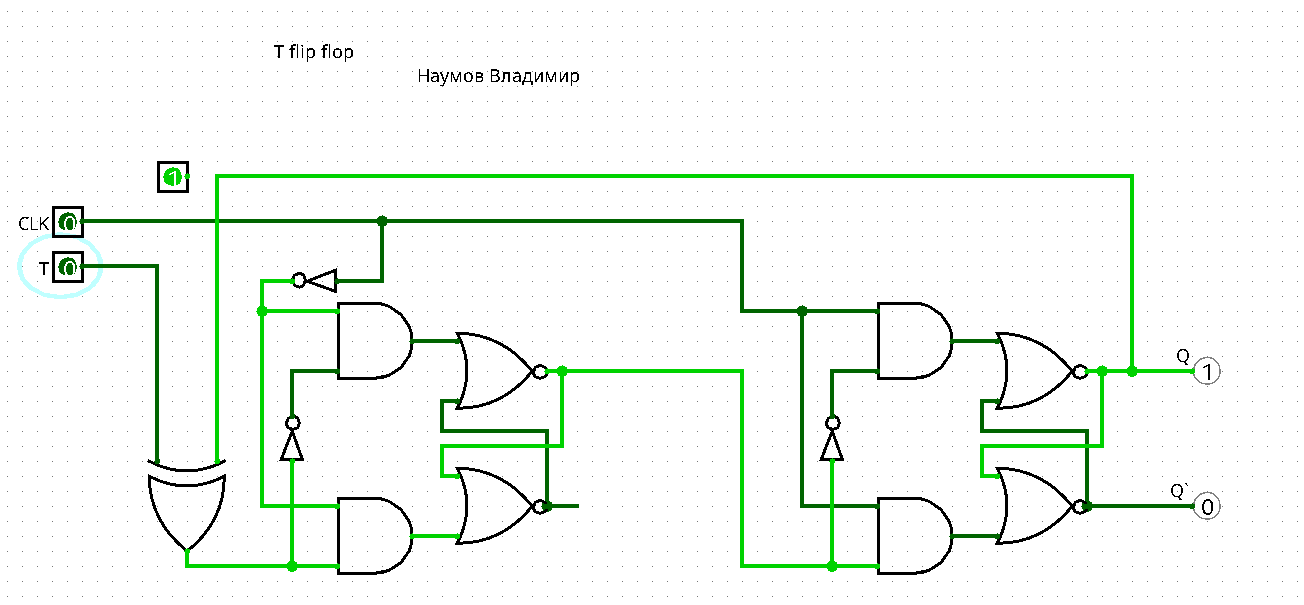
\includegraphics[width=0.8\textwidth]{state00.png}
        % \caption{Состояние 1: описание}
        \label{fig:state1}
    \end{figure}
    
    \begin{figure}[H]
        \centering
        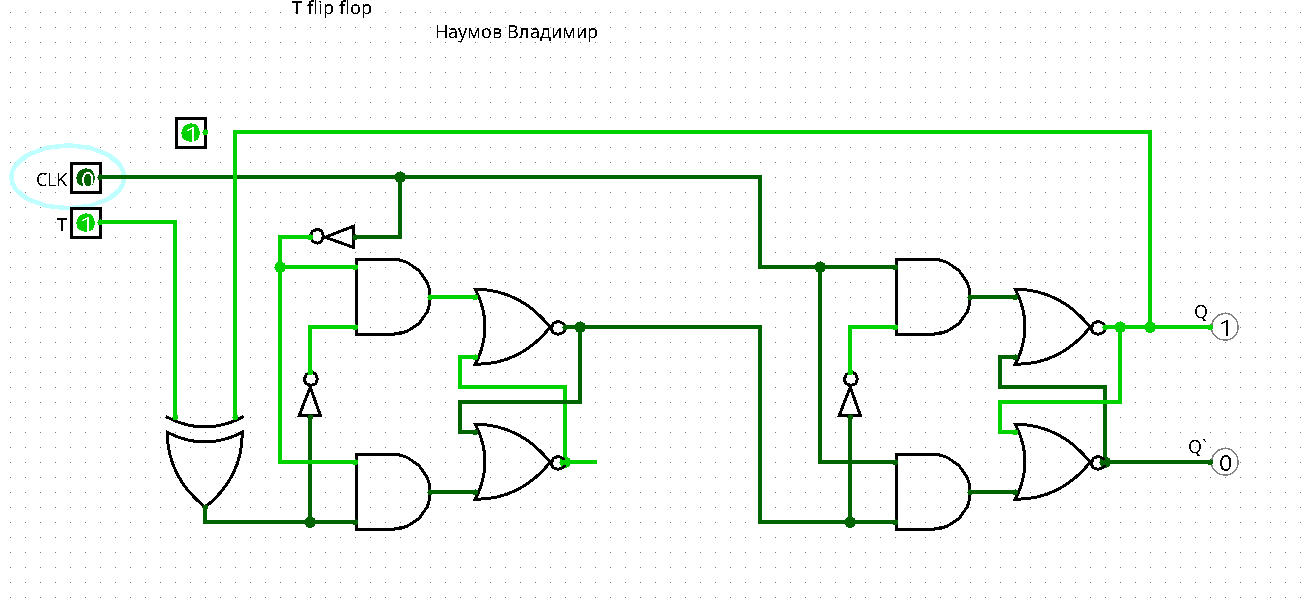
\includegraphics[width=0.8\textwidth]{state01.png}
        % \caption{Состояние 2: описание}
        \label{fig:state2}
    \end{figure}
    
    \begin{figure}[H]
        \centering
        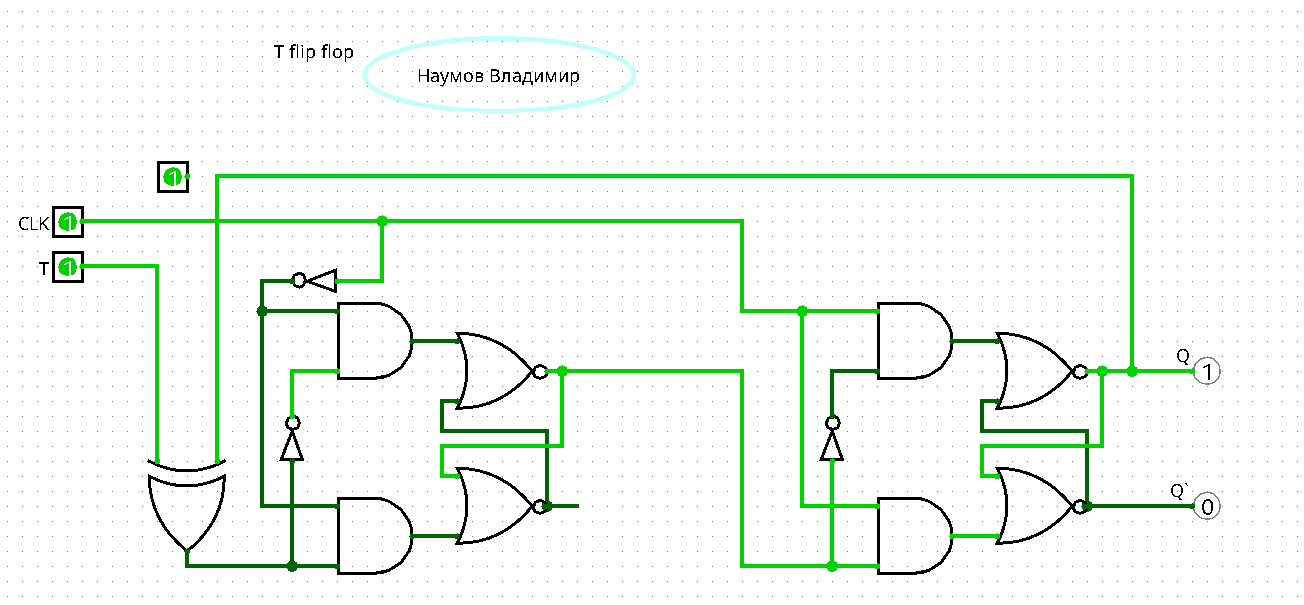
\includegraphics[width=0.8\textwidth]{state11.png}
        % \caption{Состояние 4: описание}
        \label{fig:state3}
    \end{figure}

    \begin{figure}[H]
        \centering
        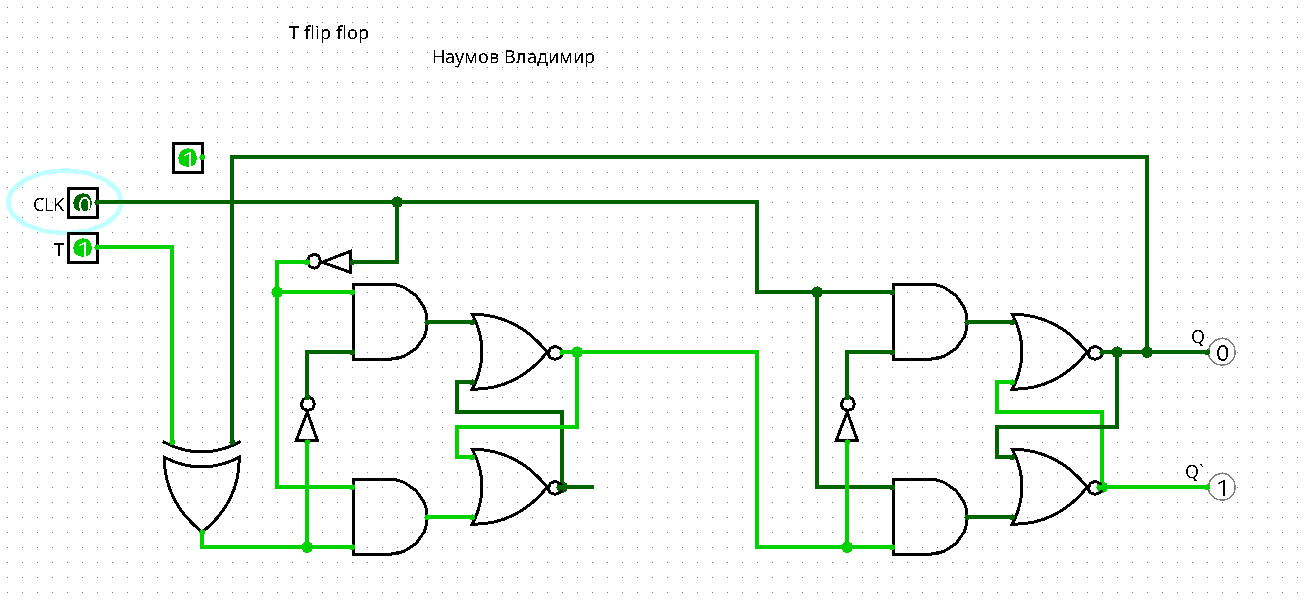
\includegraphics[width=0.8\textwidth]{state01o.png}
        % \caption{Состояние 3: описание}
        \label{fig:state3}
    \end{figure}

    \newpage
    \item \textbf{Критический путь} \\
    \begin{figure}[H]
        \centering
        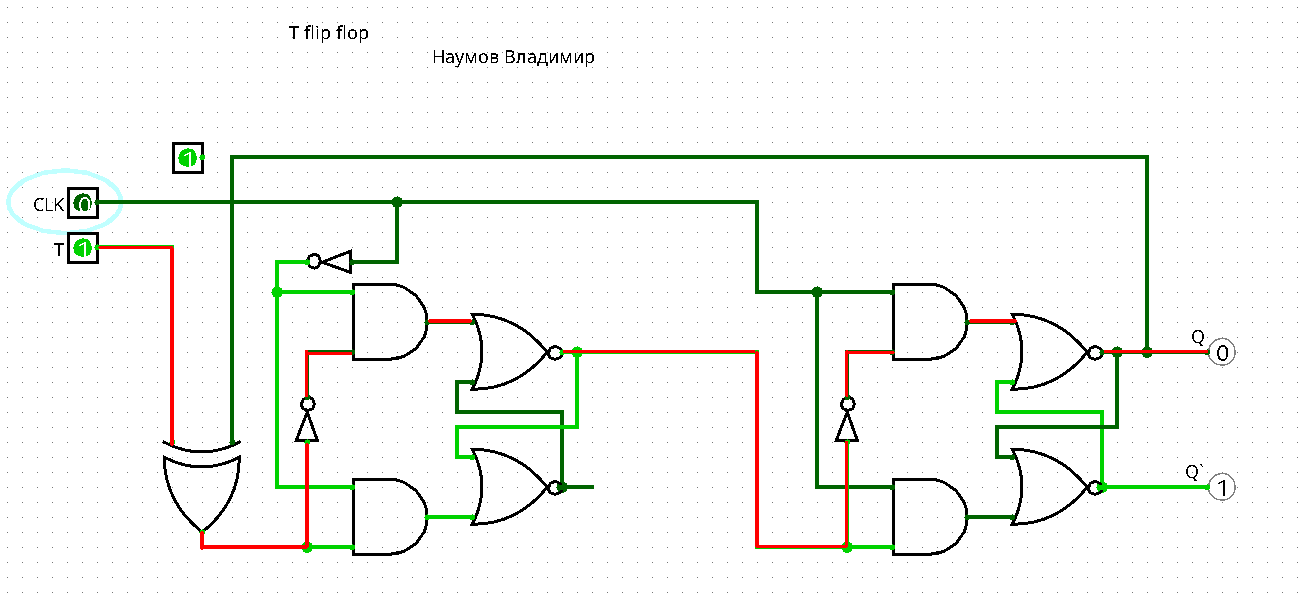
\includegraphics[width=0.8\textwidth]{critical.png}
        \caption{Критический путь (красная линия) от входа к выходу}
        \label{fig:critical}
    \end{figure}
    
    \item \textbf{Число транзисторов} \\
    Примерное число транзисторов: 62 \\
    \textbf{Подсчет:}
    \begin{itemize}
        \item NOT: 2 * 3 = 6 транзисторов
        \item AND: 4 * 6 = 24 транзистора
        \item NOR: 4 * 4 = 16 транзисторов
        \item XOR: 4 * 4 = 16 транзисторов (XOR состоит из 4-х NAND)
    \end{itemize}
\end{enumerate}
\end{document}